\documentclass{report}
\usepackage[dvipsnames]{xcolor}
\usepackage[american]{babel}
\usepackage{fontspec}
\usepackage[dvipsnames]{xcolor}
\usepackage{lmodern}
\usepackage{amssymb,amsmath}
\usepackage{comment} % enables the use of multi-line comments (\ifx \fi)
\usepackage{fullpage} % changes the margin
\usepackage{todonotes}
\usepackage{graphicx}
\usepackage{import}
\usepackage{physics}
\usepackage{systeme}
\usepackage{multicol}
\usepackage{dsfont}
\usepackage{enumitem}
\usepackage{algorithm2e}
\usepackage[lofdepth,lotdepth]{subfig}

\usepackage[backend=biber,style=apa,url=false]{biblatex}
\addbibresource{SingingBirds.bib}
\DeclareLanguageMapping{american}{american-apa}

\usepackage{xifthen}
\usepackage{soul}
\sethlcolor{Apricot}
\newcommand\bla[1]{\ifthenelse{\isempty{#1}}{\hl{**~bla~bla~**}}{\hl{**~#1~**}}}
\usepackage[unicode=true]{hyperref}
\usepackage[all]{hypcap} % ref link to the top of the figure

\usepackage{csquotes} % Dependency for APA

\usepackage{titlesec}

\titleformat{\chapter}{\normalfont\huge}{\thechapter.}{20pt}{\Huge}


\hypersetup{breaklinks=true,
            pdfauthor={Paul Ecoffet},
            pdftitle={Master thesis Computational Model of birdsong learning},
            colorlinks=true,
            citecolor=blue,
            urlcolor=blue,
            linkcolor=black,
            pdfborder={0 0 0}
            }
\urlstyle{same} % don't use monospace font for urls


\title{Master Thesis\\ Computational model of Zebra Finch song learning and the
influence of sleep on it}
\author{Paul Ecoffet\\
Supervisors: Stéphane Doncieux, Benoît Girard}
\date{The 6th of June, 2017}

\begin{document}
\maketitle

\begin{abstract}
The Zebra Finches are songbirds which learn the song of their tutor. They learn
it from 25 days post hatch (DPH) to 90 DPH \parencite{liu_juvenile_2004}. Zebra
finches are commonly used as a model of speech acquisition.

\textcite{deregnaucourt_how_2005} showed that sleep plays an important role in
the learning of tutor songs. Indeed, they showed that sleeping has a negative
impact on song restitution by zebra finches in the short term but a positive
impact on the long run. Song restitution is less complex and less similar to the
tutor song from one morning to the previous day evening, but the greater this
loss in performance was overall for one bird, the better this bird was able to
reproduce the tutor song at the end of its learning.

In addition to that, \textcite{dave_song_2000} have found neurons in the motor
cortex which fires sequences during sleep that correspond to their activity
pattern when the birds sing in adult zebra finches. This shows that motor
neurons that are highly correlated with bird's own song (BOS) are activated
during the night. These identified replays suggest that some learning may occur
during sleep that use past experiences.

Our hypothesis is that during its sleep, the zebra finch restructures the
knowledge it has acquired so far thanks to replay mechanisms. We hypothesize
that this restructuring can account for the loss of performance in the short
term and an improvement of performance in the long term.

The goal of this internship is to offer a model of the zebra finch song learning
which can explain the correlation between the loss of performance every night
and the overall performance at the end of learning.

We built a two-step learning algorithm with biological constraints that switches
between two phase. The ``day'' phase in which the algorithm tries to improve its
song production by optimizing the parameters of the motor sequence without
changing the sequence itself, and a ``night'' phase learning algorithm where the
algorithm tries to improve the sequence itself to allow the motor command to
match better the dynamics of the song without changing the parameters. We think
that modification of the sequence will have a negative impact on the short term
performance as the fit made during the day will no longer match the new
sequence, but that the new sequence will allow the day fit to match better the
tutor song as the sequence is better suited to describe the tutor song.

Our preliminary results did not confirm this hypothesis. Though, several
modifications of the models or little additions seems promising to reproduce the
effect we target.

\end{abstract}

\tableofcontents

\chapter{Introduction}\label{introduction}

\section{Zebra Finch song learning}\label{zebra-finch-song-learning}

\subsection{Characteristic of the zebra finch song
learning}\label{characteristic-of-zebra-finch-song-learning}

\todo{insert zebra finch figure}

The Zebra Finches are songbirds which learn the song of their tutor. Only males
sing and this behaviour is part of the courtship of the bird. They learn their
tutor song from 25 days post hatch (DPH) to 90 DPH \parencite{liu_juvenile_2004}
and will sing the same song for the rest of their lifes. The songs have rather
complex structures, composed of chains of syllables. A syllable is defined by a
sound surrounded by short silences. This chain of syllable is called a ``motif''
\parencite{doupe_birdsong_1999, margoliash_evaluating_2002}. Zebra finches are
close-ended learners \parencite{margoliash_sleep_2010}, they learns only one
song and will retain it their whole life, in comparison of open-ended learners
such as canaries which learns a new song each year.

The Zebra Finch learning development has been described in two different phases.
First of all, the Zebra Finch is in a sensory phase until 65DPH. During the
sensory phase, it almost does not sing and only listens to the song of its
tutor, which can be sung by a real Zebra Finch or by a song playback. This is a
critical period in which the bird memorizes fully the tutor song. Birds who have
access to the tutor song for only ten days between 25DPH and 65 DPH sing the
tutor song as good as the bird with access to the tutor song during their whole
learning \parencite{bohner_early_1990, roper_onset_2006}. The second phase is
the sensorimotor phase during which the bird sings and uses its auditory
feedback to improve its performance. Starting from 25DPH to 30DPH, the bird
produces a \emph{subsong}, a process similar to babbling. Then, the bird
produces a \emph{plastic song} starting from 50DPH. The plastic song is the
first attempts of the bird to imitate the tutor song it has memorized. Its song
productions are highly variable and become better and better copies of the tutor
song. After 90DPH, the song has reached its \emph{crystallization}. The song is
fixed and will not change throughout the Zebra Finch adulthood. The song of the
Zebra Finch gets highly stereotyped \parencite{williams_birdsong_2004}. Zebra
Finches needs auditory feedback to learn to sing. Deafening in juvenile has
severe impact on song acquisition, even if the tutor song has already been
acquired. Deafening once the song is fully learned has a much smaller impact on
performance \parencite{scharff_comparative_1991, doupe_birdsong_1999}. In
addition to that, Zebra Finches raised in isolation will also develop abnormal
songs. These two observations shows that Zebra Finches songs are acquired and
not innate. Therefore, Zebra Finches need to learn how to sing. Understanding
what mechanisms underlie this learning can help us understand what are the
prerequisites of vocal learning in others species and especially in Humans.

\subsection{Why is zebra finch song learning
studied}\label{why-is-zebra-finch-song-learning-studied}

Songbird and especially Zebra finches are commonly used as a comparison with
human about vocal development. Indeed, the song they produce are not innate even
though they have predispositions toward learning their songs. They produce
song with complex structures composed of syllables.

The neuroanatomy of Zebra Finch has also been extensively studied and the
different structures involved in singing has been identified
\parencite{nottebohm_neural_2005, bertram_two_2014}.
\textcite{doupe_birdsong_1999} even proposed parrallels between the areas
involved in song production with songbird and the areas involved in speech with
humans.

Zebra Finches are also excellent laboratory animals. They are easily
domesticated and easy to study compared to other songbirds or ``speaking''
animals\todo{not beautiful sentence}. As they learn only one song, their vocal
progress is easily trackable. The developmental trajectory can be inferred.
\textcite{deregnaucourt_how_2005} for instance tracked from the syllables
trajectories by clustering syllable productions over time.\todo{change
paragraph}

  * Well studied Neuroanatomy
  * Easy to study experimentally
        * Easily domesticated
      * Learn one song
      * Learn quickly (90DPH)
      * Easy to track song development

\section{Neurobiology of the Zebra Finch}
\label{neurobiology-of-the-zebra-finch}

\subsection{Neuroanatomy of the Zebra Finch song system}
\label{neuroanatomy-of-the-zebra-finch-song-system}

  * Connection between RA, HVC, Area X, \ldots{} Inhibition, excitation

\subsection{Pattern of activation in RA and HVC}
\label{pattern-of-activation-in-ra-and-hvc}

  * HVC clock like, temporal structure (Ali et al.)
  * RA activation while singing at very precise time and sparse coding

        * Motor control (Ali et al.) Ali et al. shows real two different
    learning: spectral and temporal

\section{Models of song learning} \label{models-of-song-learning}

Only very few models have been created. Even less are actual
computational models.

\subsection{Reinforcement learning} \label{reinforcement-learning}

  * Proposed but no real explanation of what could be the state space, the
  action space, the reward function (Dave\&Margoliash).
  * Used in paradigm to test different hypothesis (averse reward to force
  change in behaviour of the bird)

\subsection{Song preferences in selection
(Marler)} \label{song-preferences-in-selection-marler}

  * Behavioural model to explain how the bird select its template
  * TODO: Add more

\subsection{Coen's model} \label{coens-model}

  * Clustering technique with babbling (multimodal)

      * Cluster the tutor song syllables thanks to their characteristics
      * Babbling, create a mapping between the motor space and the
    identified cluster
    * Use of a real synthesizer but not actually built to model zf vocal
  apparatus
  * No quantitative means to see how good is the song reproduction
  * The learning is only babbling, nothing is driving the model in a
  specific direction.

\section{Song synthesizer}\label{song-synthesizer}

\subsection{G. B. Mindlin's song synthesizer to reproduce Zebra Finch song}
\label{description-of-perl-song-synthesizer-to-reproduce-zebra-finch-song}

\begin{figure}[htbp]
  {\center
  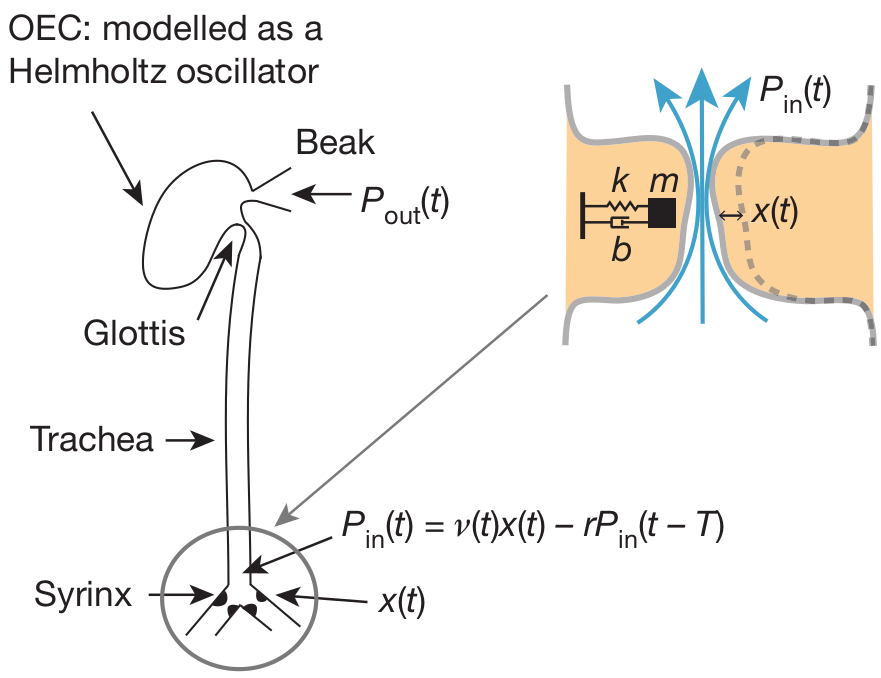
\includegraphics[width=0.5\linewidth]{media/scheme_vocal_apparatus}
  \caption{Model of the zebra finch vocal apparatus\label{zf-vocal-aparatus}}}
  \small

  The air (\(P_{sub}(t)\)) comes from the air sac below the syrinx, then goes up
  to the trachea, the glottis, resonate in the oro-esophageal cavity (OEC) and
  the beak (\(P_{out}(t)\)). Each component acts as a filter in G.B. Mindlin's
  team model of the zebra finch vocal aparatus. Figure 1b taken from
  \textcite{amador_elemental_2013}.

\end{figure}

G. B. Mindlin and his team built a model of the Zebra Finch vocal apparatus.
They described with differential equations the behaviours of the components of
this vocal apparatus (see Fig~\ref{zf-vocal-aparatus}). The differential
equations model the separation between the syringeal labia. Each labia is
modeled as a spring and mass system that can produce sustainable oscillations.
Depending of the parameters it receives, the synthesizer is able to produce a
vast variety of sounds, either very pure or very rough, depending of the
strength of the labia tension \parencite{amador_beyond_2008,
boari_automatic_2015}. The dynamic system shown in equation \ref{synth_eq_dyn}
described the mathematical simplification of their model.

\begin{equation}
\systeme*{
\dv{x}{t} = y,
\dv{y}{t} = - \alpha \gamma^2 - \beta \gamma^2 x - \gamma^2 x^3 - \gamma x^2 y
    + \gamma^2 x^2 - \gamma x y
}
\label{synth_eq_dyn}
\end{equation}

\(x\) describes the position of the syringeal labia. \(\gamma\) is a constant
which takes into account values specific for the Zebra Finch vocal apparatus.
\(\alpha\) and \(\beta\) are unit-less time-dependant parameters. \(\alpha\) is
proportional to the air sac pressure, that is how much air is coming through the
syrinx, and \(\beta\) is proportional to the syringeal labial tension. It can be
hypothesized that these two parameters can be easily modified by motor actions.
Therefore, the whole singing behaviour can be described as the dynamics of
muscles acting on the air sac pressure and the syringeal labial tension. Thus,
this synthesizer provides a way to bridge the gap between actual motor commands
and song production. Even if the model is simplified, as it assumes a symmetry
in the labial tensions, it is able to produce a rich variety of sounds.

This model of birdsong production shows that low dimensional but biologically
realistics parameters can describe the singing behaviour of the Zebra Finch.
Simple variations in the motor space produces complex and diverse variations of
the song production. This model simplifies greatly the study of song production
behaviour, as it is possible to study the dynamics of song production in the
motor space while keeping realistic constraints.

\subsection{Zebra Finches are sensible to song produced by the synthesizer}
\label{zebra-finches-are-sensible-to-song-produced-by-the-synthesizer}

The computational model of the zebra finch vocal apparatus is a real sound
synthesizer. It produces sound waves which birds, as we, can listen to. As
explained in \ref{neurobiology-of-the-zebra-finch}, Zebra Finches have neurons
which are highly selective to their BOS. When the bird is asleep and listen to
their own song, these neurons fire in a very specific pattern. To assess the
quality of their synthesizer, G.B. Mindlin team tested if their synthetical
song, built from the BOS, will activate these neurons
\parencite{amador_low_2014, boari_automatic_2015}. They showed that even if the
strenght of the activation was not as strong as the bird listening to its BOS,
their synthesized song performed better than a conspecific song or the BOS
played in reverse. This suggests that the synthesis is sufficiently good to
trick a bird. The synthesizer is thus ablet to produce good imitation of Zebra
Finch songs.

\subsection{Gestures and song structure} \label{gestures-and-song-structure}

The study of the parameters \(\alpha\) and \(\beta\) over the time course of the
song reveals interesting results. \textcite{amador_elemental_2013} propose to
describe songs by the sequence of air sac pressure (\(\alpha\)) and syringeal
labial tension (\(\beta\)) trajectories, called gestures. A gesture starts and
stops when there is a discontinuity in the trajectory of either the air sac
pressure or the tension (see Fig~\ref{gestures_schema}). If notes and syllables
are the primitives of a song in the sensory space, a gesture is the primitive of
a song in the motor space. Several subsequent gestures are needed to produce one
syllable.

Amador and her collaborators suggested that spiking pattern observed
in HVC is correlated with the onset and offset of gestures and therefore that
the HVC activity is not a clock-like pattern but the transmission of high level
motor commands which defines the song structure. This has been contested by
\textcite{lynch_rhythmic_2016} and \textcite{picardo_population-level_2016} with
extensive statistical analyses. Even if HVC neurons do not actually fire on the
onset and offset of gestures, the gesture framework is very interesting because
it allows us to think about the song structure representation in the motor
space, which is of particular interest to build a biologically plausible model
of song learning.

\begin{figure}[htbp]
  {\center
  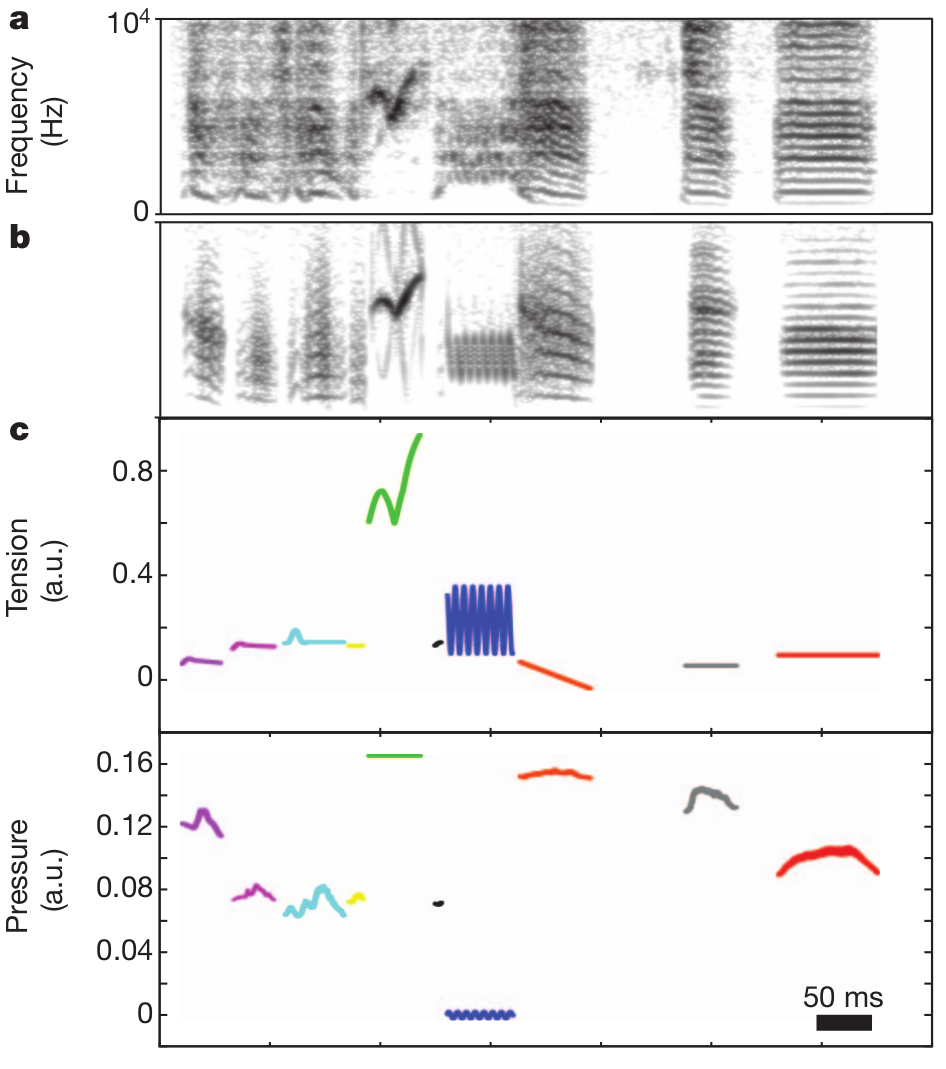
\includegraphics[width=0.5\linewidth]{media/gesture_schema_amador}
  \caption{A birdsong and its associated parameters for reproduction segmented
  in gestures\label{gestures_schema}}}

  \small
  \textbf{a)} spectrograph of a bird's song. \textbf{b)} spectrograph of the
  synthetic song. \textbf{c)} the paramaters \(\alpha\) and \(\beta\) for the
  song. There is several discontinuities in their trajectories. Each continuous
  segment forms a gesture. Figure from \textcite{amador_elemental_2013}.

\end{figure}

\section{Influence of Sleep in the Zebra Finch song development}
\label{influence-of-sleep-in-the-zebra-finch-song-development}

Several studies showed that sleep is involved in the song learning and
maintenance. \textcite{dave_song_2000} shows thanks to electrophysiology
recording the . \textcite{deregnaucourt_how_2005} showed that sleep has
\todo{complete these sentences}

\subsection{Song replays during sleep}
\label{song-replays-sleep}

As explained in the Section~\ref{neurobiology-of-the-zebra-finch}, the song
system in the zebra finch brain is highly specialized. Neurons in HVC or RA have
a very precise and stereotyped pattern of activation when the adult bird sings.
\textcite{dave_song_2000} studied the pattern of activation of RA neurons while
adult birds were asleep. They observed that neurons in RA spontaneously burst in
patterns similar to their activation patterns when the bird sings. Dave \&
Margoliash hypothesize that this replay activity could be the product of an
off-line learning mechanism. Indeed, neural replays have already been found in
the rat and it has been showed that these replays influence the construction of
its cognitive maps \parencite{de_lavilleon_explicit_2015} or that the
suppression of the replays impairs the learning
\parencite{girardeau_selective_2009}.

Dave \& Margoliash's results were obtained on adult birds which have already
learned their song. Though, we can hypothesize that RA replays also occur in the
juvenile bird and impacts its learning. The actual function of the mechanism
that produces these replays must still be determined.

\begin{figure}[tbph]
  {\center
  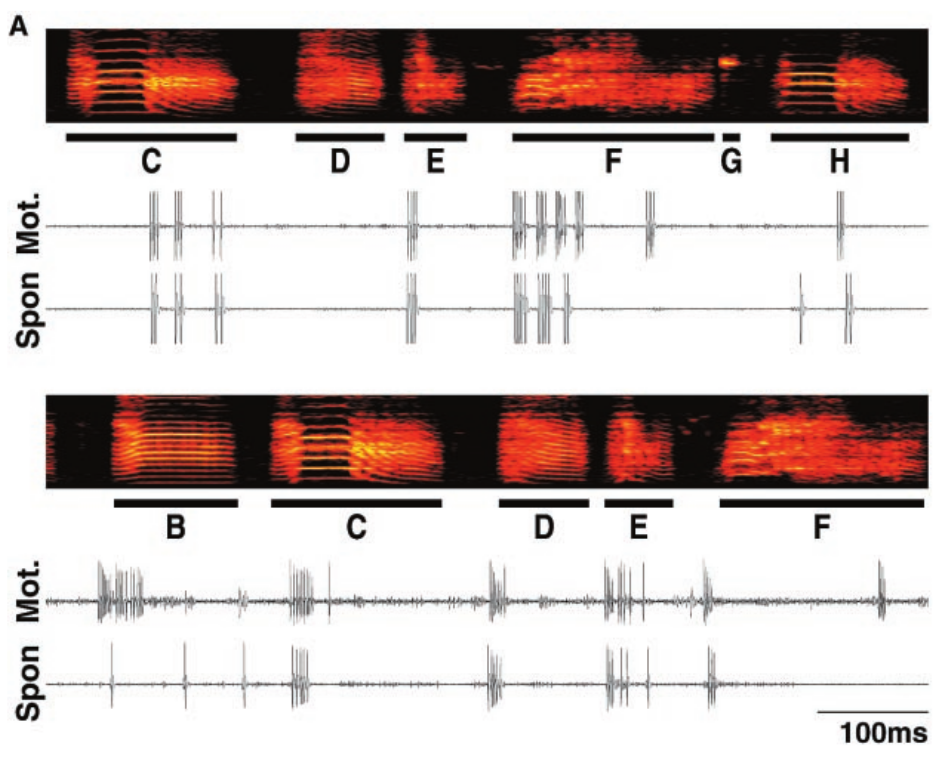
\includegraphics[width=0.7\linewidth]{media/replays_bird_margoliash}
  \caption{Neuronal replay during sleep}
  }
  \small
  Recording of the activity of two different neurons for one bird. For each
  neuron, a premotor activity is shown with the spectrograph of the BOS and the
  raw trace of a spontaneous activity during sleep that
  matches the premotor pattern. Taken from \textcite{dave_song_2000}.

\end{figure}

\subsection{The impact of sleep on the birdsong learning}
\label{impact-sleep-birdsong-learning}

\textcite{deregnaucourt_how_2005} recorded entire song developments of Zebra
Finches and studied the vocal trajectories during the whole learning process as
during the cycles of sleep and wakefulness. They tracked the development of
syllables and clustered them. Thanks to this database, they computed the shift
in the mean of the clusters for each syllable either in the same day (2 random
samples of 100 songs), from evening to the morning (last 100 songs compared to
the first 100 songs of the next day) or from the middle of one day to the middle
of the next day (random sample of 100 songs compared to a random sample of 100
songs of the next day). They computed the total vocal change for each of these
cluster, that is the relative variation of syllable features
\textcite{tchernichovski_procedure_2000}\footnote{These measures are detailled
in Section~\ref{measures}}. They found that vocal changes were the most
important with the the cluster of the evening songs compared to the next day
morning song, compared to the changes that occur for one day to the next or in
the same day (see Fig~\ref{der_abs_vocal_change}). This result shows that sleep
has a big impact in the development of the birdsong, because it cannot be
explained by the day to day vocal change.

\begin{figure}[htpb]
  {\center
  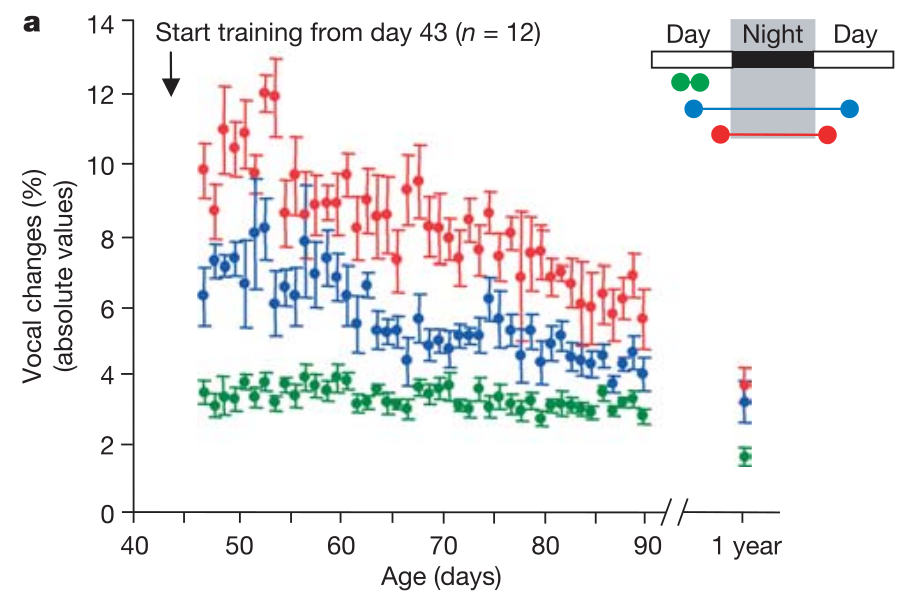
\includegraphics[width=0.7\linewidth]{media/der_absolute_vocal_change}
  \caption{Absolute vocal change during song development\label{der_abs_vocal_change}}}
  \small
  Vocal changes in absolute values (median + s.e.m). Green is the change across random sample during the same day (baseline). Blue is the change between random sample from one day to the next. Red is the vocal change from one evening to the next morning. Taken from \textcite{deregnaucourt_how_2005}.
\end{figure}

The vocal change measure Derégnaucourt and his team used is an absolute measure.
That means that this measure cannot tell if the change goes in the same trend as
the whole learning or in the opposite direction. Thus they introduce a signed
measure of vocal change. If the change goes toward the value of the feature
at the end of the learning, the signed vocal change is positive, otherwise, it
is negative. The signed vocal change showed that sleep actually has a
\emph{negative impact} on learning. Indeed, the effect of night-sleep is almost
always negative (see Fig.~\ref{der_night_signed_change}). The effect cannot be
explained by the fact the bird has not sung for a long time. Indeed, preventing
the bird of singing for 8 hours does not yield the same effect. Thus, this
unlearning is due to a mechanism which occur during sleep.

\begin{figure}[htpb]
  {\center
  \subfloat[Vocal changes in signed values during sleep]{
    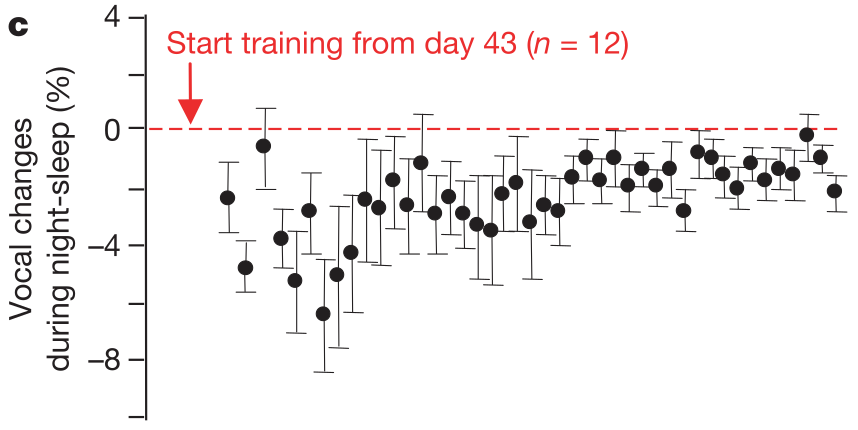
\includegraphics[height=5cm]{media/der_night_signed_change}
    \label{der_night_signed_change}
  }
  \subfloat[Entropy variance decreases during sleep]{
    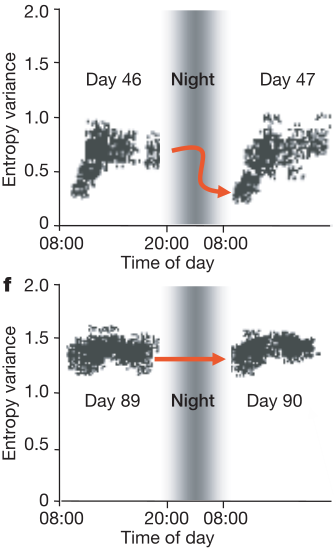
\includegraphics[height=7cm]{media/entropy_variance_night_effect}
    \label{entropy_var_night_effect}
  }
  }
  \caption{Sleep has a negative impact on vocal development}
  \small
  \textbf{a)} Vocal changes in signed values (median + s.e.m) during night-sleep compared to overall development trend.
  \textbf{b)} Entropy variance increase overall song development but decrease
  during night when the bird is still learning. At 90DPH, the bird has reach crystallisation of the song and sleep has little to no impact.
  Taken from \textcite{deregnaucourt_how_2005}.
\end{figure}

The authors computed the performance of the bird to reproduce its tutor song at
the end of its development thanks to a similarity measurement
\parencite[][developped in
section~\ref{measures}]{tchernichovski_procedure_2000}. Surprisingly, they found
that the more the post-sleep deterioration was important overall, the better the
bird was able to imitate the song of its tutor, as seen on
Fig.~\ref{der_sim_post_det}. The negative impact sleep has on learning on the
short term (day to day) has a positive impact in the long run. It shows that a
learning mechanism is at play during sleep. This learning mechanism has a
different function than the learning mechanism during the day. The authors
suggest that the oscillations in vocal learning may help the bird get out of
local maxima in development. Several learning algorithm can be investigated to
explain these results.

\begin{figure}[htpb]
  {\center
  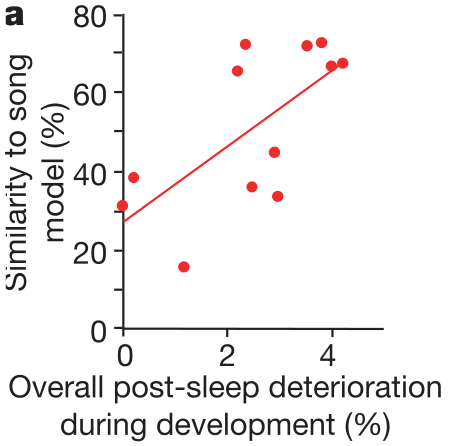
\includegraphics[width=0.3\linewidth]{media/cor_deterioration_sim}
  \caption{Correlation between post-sleep deterioration and similarity of the
  tutor song at the end of learning. \label{der_sim_post_det}}}
  \small
  The more the sleep deteriorate the bird's learning from one day to the next, the better the bird reproduces its tutor song at the end of its learning. Taken from \textcite{deregnaucourt_how_2005}.
\end{figure}


\section{A computational model of birdsong learning to explain the sleep
influence}
\label{a-computational-model-of-birdsong-learning-to-explain-the-sleep-influence}

\subsection{Interest of a computational model of birdsong learning}
\label{interest-of-a-computational-model-of-birdsong-learning}

  * Computational model helps understanding what are the \emph{implementation
  constraints} of the learning mechanisms
  * Use of synthesizer Realistic computational budget
  *Easily make hypotheses that can be tested experimentally afterwards
  Abstracted and controlled environment

\subsection{Goal: Build a modular two-step learning model and look for learning
algorithm that can account for Derégnaucourt's results.}
\label{goal-build-a-modular-two-step-learning-model}

\chapter{Our Model} \label{our-model}

The goal of this internship is to build a computational and behavioral model of
birdsong learning with realistic constraints and try to model the impact of
sleep on song development as presented in the
Section~\ref{impact-sleep-birdsong-learning}. The model is developped from
scratch in Python~3. It uses the birdsong synthesizer built by G.B.~Mindlin and
his team and the standard measures used to analyse birdsong.

The Model is a two-step learning model. The model alternates between two
different learning algorithms. The hypothesis we make is that one of
these learning algorithm correspond to the learning algorithm the bird uses
during the day, and  the second algorithm is the algorithm used by the bird
during its sleep. We hypothesize that the algorithm used during sleep should
focus on restructuration of the song models the bird has and to the diversity
\todo{}. We think that an algorithm targetting these \todo{} yields the negative
impact of sleep in the short term with a positive impact at the end of learning
as \textcite{deregnaucourt_how_2005} observed.

The source code of the model is available at
\url{https://github.com/PaulEcoffet/birdsonglearningmodel}.

\section{Global Architecture} \label{global-architecture}

The model is built in several modules. First of all, the model uses
G.B.~Mindlin's synthesizer to produce realistic song with biologically
plausible parameters (see Section~\ref{song-synthesizer}). Then, song features
measurement and songs comparison methods have been implemented and used as the
hearing system. The song feature measures were taken from the litterature
\parencite{tchernichovski_procedure_2000}. They are the standard measures used
to describe songs and syllables in the birdsong research community.

The birdsong learning model I built is a two-step learning algorithm. One
algorithm models the learning process of the bird during the day, the other
models the learning during the night. These day and night models can be easily
changed in the program I wrote.

\subsection{Boari's implementation of the birdsong synthesizer}
\label{usage-of-boaris-implementation-of-the-birdsong-synthesizer}

We want to use G.B.~Mindlin's synthesizer because it allows us to build a
computational model with realistic constraints. It bridges the gap between the
motor commands and the song production thanks to a biophysical model of the
Zebra Finch vocal apparatus. Our model can produce simple streams of \(\alpha\)
and \(\beta\) parameters and send them to the synthesizer. Then, the synthesizer
produces real sound waves that can be analyzed by the hearing system.

We use the implementation of the synthesizer available for download on the
Dynamical System laboratory of the University of Buenos Aires
(\url{http://www.lsd.df.uba.ar}) \parencite{boari_automatic_2015}. The
downloaded program was actually a combination of an \(\alpha\) and \(\beta\)
parameters extractor from an audio file and the synthesizer which can only use
the extracted parameters. I extracted the synthesizer from the source code and
adapted it so that it can receive arbitrary parameters. The synthesizer had
several bugs. It is supposed to generate a sound stream of the same length of
the parameter stream. That is, if there is 10~000 values of \(alpha\) and
\(beta\), the synthesizer should return a sound wave composed of 10~000 values.
But it actually dismiss 2 parametesr, returning only 9~998 values. As the
implementation of the synthesizer was badly documented and the source code was
not self explanatory at all, I decided to pad the \(\alpha\) \(\beta\) streams
with 2 dummy values to prevent this bug.

I have also developped a small Cython package to call Boari's C synthesizer from
Python. The source code of this package is available at
\url{https://github.com/PaulEcoffet/birdsynth}.

\subsection{Characterizing and comparing songs}

As we wanted to work on real audio signal, our algorithm must use relevant
features of the songs to describe them. Indeed, it needs to compare its
production to the tutor song so as to correct its errors and improve itself.

\subsubsection{Measurement of the song features} \label{measures}

\textcite{tchernichovski_procedure_2000} suggested several measures to
characterize Zebra Finch songs. To apply these measures, the song is first cut
into several time windows, and the measures are computed for each time windows.
These measures give us a fine-grained description of the song throughout time.

They are extensively used in the birdsong research community
\parencite{coen_learning_2007, deregnaucourt_how_2005, lipkind_stepwise_2013,
liu_juvenile_2004}.

The measure we use are the Amplitude, the Frequency Modulation, the Amplitude
Modulation, the Pitch, the Goodness and the Wiener Entropy of the signal.
Tchernikovski and his team developped a software called Sound Analysis Pro 2011
to compute these features. Though, this software runs only on Windows and its
functions cannot be called by another program. I have thus ported the
implementation of the song features measurement from a Matlab implementation
(called Sound Analysis Toolbox) to a Python implementation. The values of the
features for the same song computed by my implementation matched qualitatively
the values of the Matlab implementation (see Figure~\ref{bsa_sat_match}).

I have also reimplemented the spectral derivative plot which is
extensively used in the songbird research community to represent songs.

\todo{insert graph to show the match}

\subsubsection{Comparison of two songs}

\textcite{tchernichovski_procedure_2000} also introduced a similarity
measurement. This similarity measurement compares how a song is related to its
tutor song. To do so, the algorithm looks for matches in the features for each
sound window of the tutor song and the pupil song. The similarity score is the
percentage of the tutor song that has been matched to the pupil song. The
similarity score does not punish wrong order of syllables. For instance, if the
pupil sings the syllables A-C-B instead of A-B-C, the similarity will be very
high even if the syllables are sung in the wrong order.

Similarity is really long to compute and is only meaningful when comparing two
complete songs. It is also almost unaffected by temporal mismatches. Others
methods are used to compare syllables or notes. For simplicity, syllables are
compared by the study of means and variance of every features (Pitch, Entropy,
\ldots{}) during the syllables. Two syllables are considered similar if they
have the same mean and variance for every feature.

The Python module I wrote to compute song features and similarity scores is
called \emph{birdsonganalysis} and is available for download at
\url{https://github.com/PaulEcoffet/birdsonganalysis/}.

\subsection{Song Model}\label{song-model}

Our computational model works on the motor representations of songs. The goal of
this model is to adjust these representations so that they generate an accurate
imitation of the tutor song with G.B~Mindlin's synthesizer. I call these motor
representations \emph{Song Models}. The representation we choose for the Song
Model is highly inspired from \textcite{amador_elemental_2013} works on
gestures, as our algorithm has to feed the synthesizer with the revelant streams
of \(\alpha\) and \(\beta\) parameters. Gestures are motor primitives. They
describe simple and continuous variations of the synthesizer parameters.
Therefore, the Song Model is described as an \emph{ordered sequence} of gestures
of different durations. A gesture describes by two simple formulas the
\(\alpha\) and \(\beta\) parameters for its duration. For instance, the sequence
of a song model could be ``first, gesture A for 50~ms, then gesture B for 30~ms,
then gesture C for 120~ms''.

Be $SM$ a song model, it is defined by the $n$-uplet in equation~\ref{sm_def}.

\begin{align}
  SM &= (G_i\ \forall i = 1..n) \label{sm_def} \\
  G_i &= (Start_i, P_i)
\end{align}

With $G_i$ the $i^{th}$ gesture of the song model. $Start_i$ is the time at
which the gesture $G_i$ starts, $P_i$ are the parameters of the gesture that
describe the \(\alpha\) and \(\beta\) streams. \(Start_i < Start_{i+1} \;\forall
i\), therefore, the gestures are sequenced chronologically in the song model.
The gesture $G_i$ ends when the gesture $G_{i+1}$ starts, or when the song is
finished.

A gesture describes the \(\alpha\) and \(\beta\) streams with two formulas
parametrized by 18 values. The formulas are sums of affine and sinusoidal
functions. They are described in equations~\ref{eq_alpha} and \ref{eq_beta}.

\begin{align}
  \alpha(t) &= a_\beta \times t + b_\beta + d_\beta \sin(\omega_\beta \times 2\pi \times t + \phi_\beta) + c_\beta \label{eq_alpha} \\
  \beta(t) &= a_\alpha \times t + b_\alpha
          + \sum_{i=1}^{3} \left[ d_{i, \alpha} \sin(\omega_{i, \alpha} \times 2\pi \times t
          + \phi_{i, \alpha}) \right] + c_\alpha \label{eq_beta}
\end{align}

We choose these formulas because they roughly described the pattern of
\(\alpha\) and \(\beta\) for each gesture that we have observed using the
parameters extractor built by \textcite{boari_automatic_2015} while being still
relatively simples. Therefore, a gesture is always described by 18 parameters,
whatever its length. It greatly simplify the model as the number of parameters
to describe the song reduces massively. Indeed, he synthesizer needs an
\(\alpha\) and a \(\beta\) value at each sound sample. It means that at
44~100~Hz, to generate a sound of 20~ms (the average duration of a gesture), the
synthesizer needs 14~000 values. Our simplified formula reduces thes 14~000
values to only 18.

To simplify even more our model, we made the assumption that the song the bird
will produce matches exactly the duration of the tutor song. Therefore, the
gesture $G_i$ tries to match the tutor song starting from $Start_i$ to
$Start_{i+1}$. Be $TS$ the tutor song, we can thus define the subset $TS_i$, the
part of the tutor song that the gesture $G_i$ targets to imitate.

\begin{equation}
  TS_i = (TS(t)\ \forall t = Start_i..Start_{i+1})
\end{equation}

This is unrealistic as the pupil song timings do not exactly match the timings
of the tutor song. This constraint is due to the comparison method we choose to
assess the resemblance between the generated song and the tutor song.

All gestures at creation have the same 18 parameters (see
Appendice~\ref{all_parameters}). These inital parameters were found with grid
search to prevent the algorithm from getting stuck in either producing only
silence or only sound. Indeed, if the initial parameters produce sound, the
algorithm may not be able to find the parameters that make the synthesizer
silent, and reciprocally. The initial parameters we choose are at the boundary
between silence and phonation to avoid this issue.

\subsection{A two-step learning model} \label{two-step-learning-model}

Following the architecture of the Song Models, we notice that there are two
tasks to be fulfilled. First of all, for each gestures $G_i$, the parameters
$P_i$ must be fit so as to produce the imitation of their corresponding part
of the tutor song $TS_i$. Secondly, the gesture sequence $SM$ must be adapted so
that the gestures start and end at meaningful positions $Start_i$ and
$Start_{i+1}$. Indeed, gestures represent discontinuities of trajectory in the
motor space, therefore, the gesture onsets and offsets should be in relevant
position to produce the discontinuities needed to match the tutor song.

\todo{graphic for sequence and for parametrization of gesture}

There is therefore two algorithms that must be implemented. we can hypothesize
that one of these algorithm occurs only during day and the other only during
night. The optimization of each parameters gesture have only a positive impact
on the bird performance, but the sequence optimization could destroy the
progress of the gesture's parameters optimization by changing how the gestures
are organized. Therefore, we hypothesize that the sequence optimization
algorithm will have a negative impact on the bird performance on the short term,
but that it is needed to find the best solution and have a positive impact on
the long run. We thus think that if the parameter optimization occurs during the
day and the sequence optimization occurs during the night, we can explain the
results of \textcite{deregnaucourt_how_2005}.



\section{Day learning algorithm: Parameters
optimization}\label{day-learning-algorithm}

\subsection{Algorithm}

The goal of the day learning algorithm is to find the best parameters for each
gesture of Songs Models. We hypothesize that the bird has a small population of
concurrent Song Models to optimize, \texttt{nb\_song\_models}. Several values of
population size have been tested from 1 to 15 Song Models. We also assumed that
the bird has perfect representation of the tutor song features. It simplifies
the model and is consistent with the results of \textcite{roper_onset_2006} who
showed that the bird needs only to be exposed to the tutor song for 10 days
before the beginning of its learning to be able to reproduce it (as discussed in
Section~\ref{characteristic-of-zebra-finch-song-learning}).

The bird optimizes gesture parameters with a \emph{stochastic hillclimbing}
algorithm. The bird picks a random song model $SM_i$ to optimize, then picks a
random gesture $G_{i,j}$ from this song model. It compares the sound production
of the gesture with its actual parameters \(P_{i,j}\) to the expected result
from its tutor song memory. It then tries a small variation of every parameters
of the gesture \(P_{i, j}'\) according to a normal distribution (See
equation~\ref{draw_P}). If \(P_{i, j}'\) produces a sound matching the tutor
song better than \(P_{i, j}\), then the parameters \(P_{i, j}'\) are the new
parameters of the gesture. Otherwise, the \(P_{i_j}\) stays the gesture
parameters.

\begin{equation}
  P_{i, j}' \leftarrow P_{i, j} + \mathcal{N}(\pmb \sigma) \label{draw_P}
\end{equation}

\(\pmb \sigma\) is the covariance matrix of the parameters, and is analogeous to
the learning rate of the algorithm. Several \(\pmb \sigma\) have been tested.
They are described in the appendix \todo{}.

The process is repeated \texttt{nb\_train\_per\_day} times.

\todo{Hillclimbing figure}

\subsection{Comparison method}

To compare the song production of the gesture with the corresponding part of the
tutor song, we cannot use similarity score as it is only useful with whole songs
\parencite{tchernichovski_procedure_2000} and is computationaly very expensive
(computing the similarity between two songs takes approximatively 10 seconds).
We cannot also use the mean and variance of each song features because it makes
us lose temporal information of the production. As the gesture matches a precise
segment of the tutor song, we can compare the features of the sound window by
window between the tutor segment and the produced segment. We thus computed the
distance between these features with the following method.

Be $S_i$ the sound generated by the synthesizer with $G_i$, and $Features$ the
function that takes a signal and computes the song characteristics window by
window and returns it as a matrice $\mathcal{M}_{nb\_windows, nb\_features}$.
The distance between the two signals is computed by the formula~\ref{dist_eq}.

\begin{eqnarray}
  A = Features(S_i) - Features(TS_i) \\
  dist = \sqrt{\sum_{i=1}^{nb\_windows} \sum_{j=1}^{nb\_features} a_{i,j}^2}
  \label{dist_eq}
\end{eqnarray}

Note that we can do that only because we hypothesized that a Song Model tries to
match exactly the tutor song timing as explained in section~\ref{song-model}.
Other methods of comparison such as Dynamic Time Warping can be investigated to
allow a more flexible timing in the Song Model. We used a fixed duration
distance for simplicity.

The goal of the hillclimbing algorithm is to minimize $dist$ for each $G_{i,j}$.

\subsection{Synthesizer issues}

The production of the whole song by the synthesizer is rather long. It takes
approximately 1 or 2 seconds of computational time to produce 1 second of song.
So as to improve the performance of the program, I decided to generate only the
sound of the gesture and to compare it with its corresponding tutor song part.
G.B.~Mindlin's synthesizer is not highly influenced by its previous state,
although it seems to have a few fixed oscillatory patterns that create phase
dependant problems. For instance, be $S(\alpha, \beta)$ the sound signal
generated by the synthesizer, we have slightly different results in phase when
we generate $S(\alpha_{whole\_song}, \beta_{whole\_song})$, extract the sound
from $Start_i$ to $Start_{i+1}$ and compare it to $S_i$. These slightly
different phases have an impact on the song feature measurements (see
Figure~\ref{perf_loss}). Therefore, new gesture parameters can improve the song
imitation for a partial generation of the songbut impact negatively the whole
song production. Loss of performance can happen due to this issue. As the speed
gain from the partial generation of the song is massive, I keep it in the model.
Sadly, the loss in performance due to this bug is too common and we plan to fix
it for future simulations.

\todo{figure showing the small differences in measurements}

Nonetheless, our prediction with the day learning algorithm is that it will have
a positive impact on performance every day. Though, as the gesture sequence may
not be adapted to describe the motor commands needed to imitate the song, and as
the hillclimbing algorithm always tries to locally improve the song imitation,
the bird should get stuck in local optima. The bird can no longer improve its
performance once in a local optima, even though it is far from reproducing a
good copy of the song\footnote{Note that we cannot test this prediction before
having corrected the issues explained above}. The bird also needs to improve
the gesture sequences of its Song Models to produce accurate imitation of the
tutor song.

\section{Night learning algorithms: Sequence Optimization}
\label{night-learning-algorithms}

We hypothesize that the sequence optimization algorithm occurs during the bird's
sleep. We think that sequence optimization can explain Derégnaucourt's results
showing that sleep has a negative impact on performance in the short term but a
positive impact on the long term. Indeed, the bird needs to know when he must
change its motor trajectory, if the sound it targets must be described in more
gestures, or the gesture to produce a targeted sound must be shorter or longer.
Modifying the gesture sequence without changing gesture parameters must
negatively impact the performance, as the parameters were picked for a sequence
which no longer correspond to their target. The presence of replays of song
motor commands during sleep suggests that the bird works on the motor patterns
of its song. This corroborate our hypothesis that the bird has access to the
song representations when it sleeps.

Evolutionary algorithms are amongst the simplest algorithms to optimize a
sequence \todo{not really a good source}\parencite{eiben_introduction_2003}.Our
algorithm takes the population of Song Models from the day learning algorithm.
It then extends this population to a size of \texttt{nb\_song\_models\_night} by
creating new Song Models that are sequence variations of the day Song Models.
The increase in population allows more diversity in the sequences and thus a
better exploration of the possible sequences adapted for the reproducing the
tutor song.

The variation of a sequence can be done with several rules. The algorithm can
either insert a new gesture between two gestures, remove a gesture, change the
duration of a gesture, copy the gesture parameters of a gesture to another
gesture, or simply do nothing.

The new Song Models are then evaluated. The worst Song Models are replaced with
variations of the best Song Models.

Then, \texttt{nb\_song\_models} Song Models are selected to be the next day
Song Models. They can be picked either by random or by selecting the best Song
Models, depending on the simulation parameters.

\subsection{Microbial Genetic Algorithm}
\label{mga}

We used a variation of the Microbial Genetic Algorithm as our night learning
algorithm. The Microbial Genetic Algorithm is one of the simplest evolutionary
algorithm. Two random individuals of the population are compared according to a
criterion in a tournament. The winner of the tournament stays in the population,
and the loser of the tournament is replaced by a variation of the winner.
Therefore, the most accurate descriptions of the gesture sequence propagates in
the population while poor descripitions are forgotten. The algorithm does
\texttt{nb\_tournaments} tournaments each time it is run. We hypothesize that
the amount of tournaments should be in the same order of magnitude as the amount
of replays observed during sleep. Indeed, a tournament need Song Models
activations, so the patterns that represent them must be activated too.

We choose to use the same criterion as for the day learning algorithm. The Song
Model that wins a match is the one that has the lowest \(dist\) with the tutor
song. The underlying hypothesis is that the bird is able during its sleep to
infer what would be the effect of the gesture sequence modification on its song
production without any auditory feedback.

Even if we still select on the song reproduction quality, we hypothesize that
the sequence variation generates nonetheless loss in performances. We also
hypothesize that an explicit maintenance of \emph{diversity} in the population
would produce a even stronger loss in performance in the short term and improve
in performance on the long term. Indeed, evolutionary algorithm can get stucked
in local optima because only one kind of solution has propagated in the whole
population. Small variation of the best solution are always less performant. The
idea of diversity is to encourage different solutions even if they are less good
than the other individuals. Diversity is a way of encouraging exploration
instead of exploitation of the best solutions
\parencite{eiben_introduction_2003}. The most different individuals explore
whole new sequences that have the room to be improved so as to outpass the
actual best sequences. This method is a multi-objective optimisation which
minimise distance and maximise diversity.

I implemented the explicit diversity maintenance by punishing the Song Models
that have too much neighbours. Song Model \(SM_j\) is a neighbour of \(SM_i\)
if they have a sequence of gestures close to the sequence of \(SM_i\). I decided
to measure it by the closeness of the onset of each gesture between Song Models.
Be \(Seqdist(SM_i, SM_j)\) the sequence distance between two song models.

\begin{equation}
  Seqdist(SM_i, SM_j) = \sum_{k=0}^{nb\_gestures\_SM_i}
      \min_{l \in 0..nb\_gestures\_SM_j}(|Start_{i,k} - Start_{j, l}|)
\end{equation}

\(SM_i\) and \(SM_j\) are considered neighbour if $Seqdist(SM_i, SM_j) < th$,
$th$ a fixed threshold.

For each $SM_i$, the algorithm compute the number of neighbours it has and then
multiply the distance between the song model production and the tutor score with
the number of neighbours. It is a variation of what is found in the literature
for maximisation of a score with diversity where the score is divided by the
number of neighbours. Here, as we try to minimize the score, we punish by
multiplication. Be $score_i$ the score of $SM_i$.

\begin{align}
  neighbours_i &= \sum_{j=1}^{nb\_song\_models\_night}
  \mathds{1}_{Seqdist(SM_i, SM_j) < th} \\
  score_i &= dist(SM_i, TS) \times neighbours_i
\end{align}

In a tournament, the winner is the Song Model with the lowest score.
\texttt{nb\_tournaments} are made for each night learning algorithm run.

\todo{insert figure from poster of algorithm}

We predict that the structure variations yield a loss in performance on the
short term because the gestures parameters are no longer adapted to the new
structure. We also hypothesize that the diversity criterion makes the effect
even stronger, as it will discard more good performance in favor of more
exploration of the sequence space. This exploration allows the discovery of more
adapted sequences that are not fit yet. Therefore, this algorithm should
reproduce \textcite{deregnaucourt_how_2005} observations about the influence of
sleep on song development.

\section{Parameters} \label{parameters}

  * Tried to be realistic
  * most are fit through gridsearch
  * Realistics: Number of days, number of syllables sung during all dev
  * Gridsearch optimization
  * Default value for gesture parameters
  * Learning rate
        * Prevent part of unlearing
      * Could be fit to match real song learning rate
      * Coefficient for score optimization
    * Algorithm way better in score than Boari but qualitatively very
  different to the ear
  * Look at which parameters boari's method was better than algo and put
  priority on them
  * Amplitude and entropy
  * Diversity threshold to maximise variance in diversity score

        * Value: 5000
      * Other parameters
    * Number of song models during day and night: Depend of runs
  * Boundaries for parameters values: Fixed
  * Number of tournaments during night: depend of runs
        * Correlated with replay? By how much?

\chapter{Analyses and results}\label{analyses-and-results}


\section{Learning method is as good Boari's method or
better}\label{learning-method-is-as-good-boaris-method-or-better}

My model is able to reproduce accurately birdsongs. According to the comparison
method I use, the reproduction of the song is as good or better

  * Using standard measure criteria in the birdsong community
  * Simple description of motor params sufficient to produce good songs
  * Qualitatively same amount of gestures
        * Can be due to luck

  \section{Too little training per model cause
divergence}\label{too-little-training-per-model-cause-divergence}

  * maybe due to global vs local error

\section{Derégnaucourt results not
reproduced}\label{deruxe9gnaucourt-results-not-reproduced}

  * Syllables extracted by time of begin and end
  * Without or with diversity
  * No night deterioration
  * Night deterioration has no impact in overall learning


\chapter{Discussion}\label{discussion}

\section{The synthesizer which cannot produce every
sounds}\label{the-synthesizer-which-cannot-produce-every-sounds}

  * Our score really close to boari's method (not way better or way
  worst), maybe we reached synthesizer limits

\section{The parameters description we choose}
\label{the-parameters-description-we-choose}

  * more simple/complexe possible than sum of sin and affine?
\section{The unlearning during day due to the gesture
learning}\label{the-unlearning-during-day-due-to-the-gesture-learning}

\section{Fixed duration of songs in
learning}\label{fixed-duration-of-songs-in-learning}

  * Dynamic Time Warping can correct that
\section{Big artificial separation between structuration and gestures
optimization}\label{big-artificial-separation-between-structuration-and-gestures-optimization}

\section{Diversity not strong enough? What if only diversity during
night?}\label{diversity-not-strong-enough-what-if-only-diversity-during-night}

  * Maybe not convergence
  * Maybe what we are looking for
\chapter{Conclusion}\label{conclusion}

\section{Learning algorithm with two step
learning}\label{learning-algorithm-with-two-step-learning}

  * Very few of them
  * Working with realistic synthesizer
  * modular architecture, easy to test new models
\section{Restructuration didn't yield the expected
effect}\label{restructuration-didnt-yield-the-expected-effect}

 * More parameters search might be able to fix it

\printbibliography{}

\end{document}
